%
% Modo de operación CBC, capítulo de antecedentes.
% Proyecto Lovelace.
%

\subsection{\textit{Cipher-block Chaining} (CBC)}

En CBC la salida del bloque cifrador uno se introduce (junto con el siguiente
bloque del mensaje) en el bloque cifrador dos, y así en sucesivo. Para poder
replicar este comportamiento en todos los bloque cifradores, este modo de
operación necesita un argumento extra a la entrada: un vector de
inicialización. De esta manera la salida del bloque $ i $ depende de todos
los bloques anteriores; esto incrementa la seguridad con respecto a ECB.

\vspace{0.5cm}

\begin{figure}[H]
  \centering
  \begin{subfigure}{0.45\textwidth}
      \begin{center}
          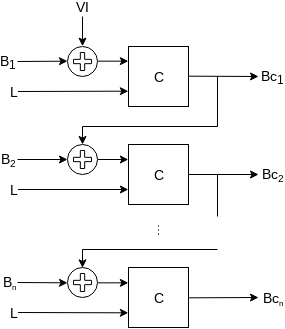
\includegraphics[width=0.7\linewidth]
            {contenidos/antecedentes/modos/diagramas/modo_cbc.png}
          \caption{Cifrado.}
      \end{center}
  \end{subfigure}
  \begin{subfigure}{0.45\textwidth}
      \begin{center}
          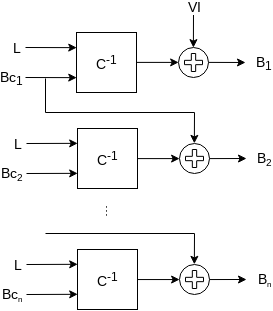
\includegraphics[width=0.7\linewidth]
            {contenidos/antecedentes/modos/diagramas/modo_cbc_inverso.png}
          \caption{Descifrado.}
      \end{center}
  \end{subfigure}
  \caption{Modo de operación CBC.}
  \label{figura:cbc}
\end{figure}

En la figura \ref{figura:cbc} se muestran los diagramas esquemáticos para
cifrar y descifrar; en los pseudocódigos \ref{cbc:1} y \ref{cbc:2} se muestran
unos de los posibles algoritmos a seguir. Es importante notar que mientras que
el proceso de cifrado debe ser forzosamente secuencial (por la dependencias
entre salidas), el proceso de descifrado puede ser ejecutado en paralelo.

\vspace{0.5cm}

% Látima que con los escapes en modo matemático dentro de los pseudocódigos
% se pierda totalmente la ventaja de trabajar con fuentes mono: por eso
% la alineación tan rara de los comentarios del próximo pseudocódigo.

\begin{pseudocodigo}[caption={Modo de operación CBC, cifrado.}, label={cbc:1}]
  entrada: llave $ L $; vector de inicialización $ VI $;
           bloques de mensaje $ B_1, B_2 \dots B_n $.
   salida: bloques de mensaje cifrado $ Bc_1, Bc_2 \dots Bc_n $.
  inicio
    $Bc_0$ $\gets$ $ VI $                         // El vector de incialización
    para_todo $B$                 // entra al primer bloque.
      $Bc_i$ $\gets$ C($L$, $B_i \oplus Bc_{i - 1}$)
    fin
    regresar $Bc$
  fin
\end{pseudocodigo}

\begin{pseudocodigo}[caption={Modo de operación CBC, descifrado.}, label={cbc:2}]
  entrada: llave $ L $; vector de inicialización $ VI $;
           bloques de mensaje cifrado $ Bc_1, Bc_2 \dots Bc_n $.
   salida: bloques de mensaje original $ B_1, B_2 \dots B_n $.
  inicio
    $Bc_0$ $\gets$ $ VI $
    para_todo $Bc$
      $B_i$ $\gets$ $C^{-1}$($L$, $Bc_i$) $\oplus$ $Bc_{i-1}$
    fin
    regresar $B$
  fin
\end{pseudocodigo}
